\documentclass[10pt,a4paper]{article}
\usepackage[latin1]{inputenc}
\usepackage{amsmath}
\usepackage{amsfonts}
\usepackage{amssymb}
\usepackage{makeidx}
\usepackage{graphicx}
\author{Artem Los}
\title{Hello}

\usepackage{marginnote}
\usepackage{verbatim} % for the box
\usepackage{fancyvrb} % for the box

\usepackage{listings}

\lstset{language=Java,
numberstyle=\footnotesize,
basicstyle=\ttfamily\footnotesize,
numbers=left,
rulesepcolor=\color{gray}, %fancy shadow for borders
stepnumber=1,
frame=shadowbox,
breaklines=true}

\usepackage{pgf}
\usepackage{pgfpages}

\usepackage{fullpage}  % might require you to compile the page several times.



\begin{document}

\section*{Exercise 3.1}

\begin{figure}[h]
\center
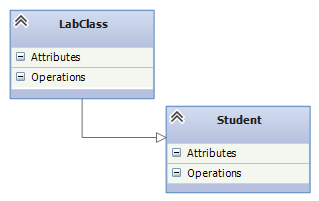
\includegraphics{rel1}
\caption{Class diagram}
\end{figure}
\begin{figure}[h]
\center
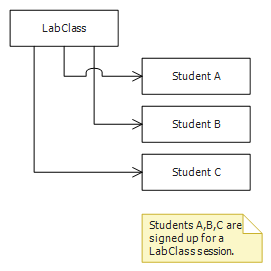
\includegraphics{rel2}
\caption{Object diagram}
\end{figure}
A class diagram illustrates the relationship between classes in general. As it can be seen in Figure 1, we can see that Student class is a part of a Lab class. An object diagram, in contrast to a class diagram, displays the way objects look like at a certain point in the objects' lifecycle. Figure 2 clearly shows that in that particular case, there are three Student objects that have signed up for a Lab Class session.

\section*{Exercise 3.2}
A class diagram can change when the class is changed or the way the classes are connected. So, if we add a new field to the Lab Class or add a new class, \textit{School} that will be a superset of Lab Class, the class diagram will change.

\section*{Exercise 3.3}
An object diagram change anytime the objects change. So, if we add more students to a lab session, the object diagram will change too. 


\section*{Exercise 3.9}
The following are going to be true:
\begin{itemize}
\item \verb|!false|
\item \verb|(34!=33) && !false|
\end{itemize}

\section*{Exercise 3.10}
True for \textbf{a} and \textbf{b} when either both are \textit{true} or both are \textit{false}.

\begin{lstlisting}
a && b || !a && !b
\end{lstlisting}

\section*{Exercise 3.11}
True for \textbf{a} and \textbf{b} when either one is true but not both.

\begin{lstlisting}
a ^ b
\end{lstlisting}

\section*{Exercise 3.12}
\begin{lstlisting}
! (!a || !b)
\end{lstlisting}

\section*{Exercise 3.21}
The increment method can either be written as
\begin{lstlisting}
int x = (value +1);
value = x - limit * (x/limit) ;
\end{lstlisting}
or, using an if statement
\begin{lstlisting}
int x = value +1;
        
if(x < limit)
{
    value = x;
}
else
{
    value = 0;
}
\end{lstlisting}
$\therefore$ The modulo operator is better than either of these methods since it does not involve so many lines of code. We do not need to consider the formal definition of mod each time we want to use it, so instead we can focus on the complex logic.

\section*{Exercise 3.26}
\begin{lstlisting}
public Editor(string fileName, int x)
\end{lstlisting}

\section*{Exercise 3.27}
\begin{lstlisting}
Rectangle window;
Rectangle rectangle = new Rectangle(3,2);
window = rectangle;
\end{lstlisting}

\section*{Exercise 3.30}
\begin{lstlisting}
p1.print("helloworld.txt", true);
p1.getStatus(30);
\end{lstlisting}

\section*{Exercise 3.31}
The \textbf{ClockDisplay} class
\begin{lstlisting}
public class ClockDisplay
{
    private NumberDisplay hours;
    private NumberDisplay minutes;
    private String displayString;    // simulates the actual display
    private boolean pm = false;
    
    public ClockDisplay()
    {
        hours = new NumberDisplay(13,1);
        minutes = new NumberDisplay(60);
        updateDisplay();
    }


    public ClockDisplay(int hour, int minute)
    {
        hours = new NumberDisplay(13, 1);
        minutes = new NumberDisplay(60);
        setTime(hour-1, minute);
    }


    public void timeTick()
    {
        minutes.increment();
        if(minutes.getValue() == 0) {  // it just rolled over!
            hours.increment();
            
            if(hours.getValue() == 12)
            {
                pm = ! pm;
                hours.setValue(0);
            }
        }
        
        updateDisplay();
    }


    public void setTime(int hour, int minute)
    {
        hours.setValue(hour);
        minutes.setValue(minute);
        updateDisplay();
    }


    public String getTime()
    {
        return displayString;
    }
    

    private void updateDisplay()
    {
        displayString = hours.getDisplayValue()+  ":" + 
                        minutes.getDisplayValue() + (pm  ? "pm" : "am");
    }
}

\end{lstlisting}

The \textbf{NumberDisplay} class
\begin{lstlisting}
public class NumberDisplay
{
    private int limit;
    private int value;
    private int startingIndex;

    public NumberDisplay(int rollOverLimit)
    {
        limit = rollOverLimit;
        value = 0;
        startingIndex = 0;
    }
    
    public NumberDisplay(int rollOverLimit, int _startingIndex)
    {
        limit = rollOverLimit;
        value = 0;
        startingIndex = _startingIndex;
    }


    public int getValue()
    {
        return value;
    }

    public String getDisplayValue()
    {
        int temp = value + startingIndex;
        if(value < 10) {
            return "0" + temp;
        }
        else {
            return "" + temp;
        }
    }


    public void setValue(int replacementValue)
    {
        if((replacementValue >= 0) && (replacementValue < limit)) {
            value = replacementValue;
        }
    }


    public void increment()
    {
        value = (value + 1) % limit;
    }
}


\end{lstlisting}

\section*{Exercise 3.32}
In \textit{Exercise 3.31} and \textit{Exercise 3.32}, two ways of constructing a 12-hour based clocks are presented. To answer the question which is better, we must define what is to be valued more in both situations.    I think it all depends on the time we want to put into it. It took longer for me to construct the clock in \textit{Exercise 3.31} in comparison to \textit{Exercise  3.32}. Personally, I would go with \textit{Exercise 3.32}, since, in terms of mathematics, much easier. A 12 hours based  clock requires modulo arithmetic with some minor changes, as we do not allow zero. In a 24 hour based clock, maths is easier since zero is included.

The \textbf{ClockDisplay} class.
\begin{lstlisting}
public class ClockDisplay
{
    private NumberDisplay hours;
    private NumberDisplay minutes;
    private String displayString;    // simulates the actual display
    
    public ClockDisplay()
    {
        hours = new NumberDisplay(24);
        minutes = new NumberDisplay(60);
        updateDisplay();
    }

    public ClockDisplay(int hour, int minute)
    {
        hours = new NumberDisplay(24);
        minutes = new NumberDisplay(60);
        setTime(hour, minute);
    }


    public void timeTick()
    {
        minutes.increment();
        if(minutes.getValue() == 0) {  // it just rolled over!
            hours.increment();
        }
        updateDisplay();
    }


    public void setTime(int hour, int minute)
    {
        hours.setValue(hour);
        minutes.setValue(minute);
        updateDisplay();
    }

    public String getTime()
    {
        return displayString;
    }
    
    private void updateDisplay()
    {
        int temp = hours.getValue ();
        
        hours.setValue(temp % 12 +1);
        
        displayString = hours.getDisplayValue() + ":" + 
                        minutes.getDisplayValue() + (temp/12 > 0 ? "pm" : "am");
                        
       hours.setValue(temp);
    }
}
\end{lstlisting}

The \textbf{NumberDisplay} class.
\begin{lstlisting}

/**
 * The NumberDisplay class represents a digital number display that can hold
 * values from zero to a given limit. The limit can be specified when creating
 * the display. The values range from zero (inclusive) to limit-1. If used,
 * for example, for the seconds on a digital clock, the limit would be 60, 
 * resulting in display values from 0 to 59. When incremented, the display 
 * automatically rolls over to zero when reaching the limit.
 * 
 * @author Michael Kölling and David J. Barnes
 * @version 2011.07.31
 */
public class NumberDisplay
{
    private int limit;
    private int value;

    /**
     * Constructor for objects of class NumberDisplay.
     * Set the limit at which the display rolls over.
     */
    public NumberDisplay(int rollOverLimit)
    {
        limit = rollOverLimit;
        value = 0;
    }

    /**
     * Return the current value.
     */
    public int getValue()
    {
        return value;
    }

    /**
     * Return the display value (that is, the current value as a two-digit
     * String. If the value is less than ten, it will be padded with a leading
     * zero).
     */
    public String getDisplayValue()
    {
        if(value < 10) {
            return "0" + value;
        }
        else {
            return "" + value;
        }
    }

    /**
     * Set the value of the display to the new specified value. If the new
     * value is less than zero or over the limit, do nothing.
     */
    public void setValue(int replacementValue)
    {
        if((replacementValue >= 0) && (replacementValue < limit)) {
            value = replacementValue;
        }
    }

    /**
     * Increment the display value by one, rolling over to zero if the
     * limit is reached.
     */
    public void increment()
    {
        value = (value + 1) % limit;
    }
}
\end{lstlisting}

\section*{Exercise 3.34}
The object diagram of the \textit{Mail Server} and three \textit{Mail Clients}.
\begin{figure}[h]
\center
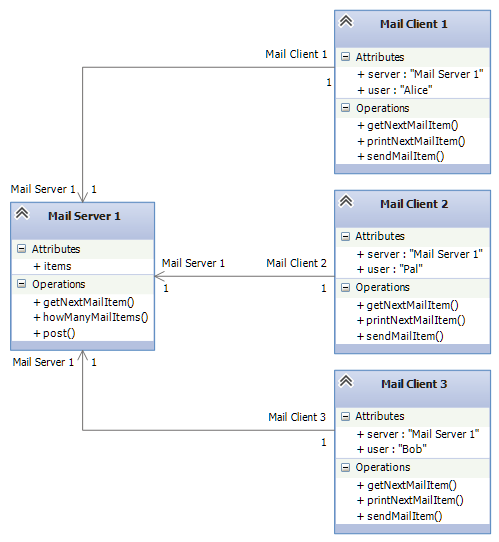
\includegraphics{rel3}
\caption{The arrow from Mail Clients is drawn because each Mail Client is connected to a certain server. The field "server" in each Mail Client takes care of the server.}
\end{figure}
\end{document}

